% ch1.tex
% This work is licensed under the Creative Commons Attribution-Noncommercial-Share Alike 3.0 New Zealand License.
% To view a copy of this license, visit http://creativecommons.org/licenses/by-nc-sa/3.0/nz
% or send a letter to Creative Commons, 171 Second Street, Suite 300, San Francisco, California, 94105, USA.


\chapter{Не все змеи кусаются}\label{ch:notallsnakeswillsquishyou}

Скорее всего, ты получил эту книгу на день рождения. Или, возможно, на Новый Год. Тётя Надя собиралась подарить тебе два разных носка огромного размера (которые ты не захотел бы носить даже, когда вырастешь). Вместо этого, она услышала чей-то разговор о книжке, которую можно напечатать, и вспомнив, что у тебя был один из этих компьютеров, которым ты пытался научить ее пользоваться в прошлый Новый Год (ты сдался, когда она стала пытаться разговаривать с мышкой), попросила распечатать ей ещё одну копию книги. Просто будь благодарен, что не получил те замшелые старые носки.

Я надеюсь, ты не слишком разочарован тем, что это я выскочила из подарочной упаковки, вместо тех носков. Не слишком уж разговорчивая (ладно, совсем не разговаривающая) книга, со зловещщего вида названием на обложке про ``Изучение $\ldots$''.
Но задумайся на минутку о моих чувствах. Если бы ты был героем одного из романов про волшебников, что стоят в твоем книжном шкафу, у меня, вероятно, были бы зубы... или даже глаза. У меня внутри были бы движущиеся картинки, или я бы издавала всякие стонущие и зывывающие звуки, когда ты перелистываешь мои страницы. Вместо этого я распечатана на листах обычной бумаги формата А4 с помятыми уголками, сшитых степлером или засунутых в папку. Хотя, откуда бы мне знать---у меня же нет глаз.
\\
\\
\emph{Эх, я бы все отдала за комплект хороших, острых зубов$\ldots$}
\\
\\
Однако, всё не так плохо, как кажется. Хоть я и не могу говорить ... или кусать за пальцы, когда ты отворачиваешься... Я могу рассказать тебе немного о том, что заставляет компьютеры работать. Не физически, благодаря проводам, микросхемам, кабелям и устройствам, которые, наверняка, ударят тебя током, если ты прикоснешся к ним (поэтому, не трогай!!)---а про скрытые штуки, те, что работают внутри всех этих проводов, микросхем и кабелей и делают компьютеры по настоящему полезными.

\begin{wrapfigure}{r}{0.5\textwidth}
  \begin{center}
    \includegraphics*[width=70mm]{electrocute.eps}
  \end{center}
\end{wrapfigure}

Это немного похоже на мысли, бегающие внутри твоей головы. Если бы у тебя не было мыслей, ты бы сидел на полу своей спальни, рассеяно глядя на дверь, и пускал слюни на свою футболку. Без \emph{программ}, компьютеры были бы полезны только в качестве подставки для ног---и даже тогда они были бы не слишком полезны, потому что ты бы постоянно спотыкался об них по ночам. Ведь нет ничего хуже, чем удариться ногой в темноте.
\\
\\
\emph{Я всего лишь книга, но даже я знаю это. }
\\
\\
У твоей семьи может быть Playstation, Xbox или Wii, стоящий в гостиной - они не используются без программ(игр) которые для них сделали. Ваш DVD-плеер, возможно, ваш холодильник и даже ваша машина - всё имеет компьютерные программы, которые делают эти вещи более полезными, чем они были бы без таких программ. Ваш DVD-плеер имеет программу позволяющую проиграть изображение записанное на DVD; ваш холодильник имеет программу, контролирующую потребление электричества, но позволяющую оставаться еде холодной; ваша машина возможно имеет компьютер, который предупреждает водителя об опасности.\\
Если вы знаете, как писать компьютерные программы, вы можете делать разные полезные штуки. Возможно, писать свои собственные игры. Создавать web страницы, которые действительно делают что-то полезное, а не просто красиво смотрятся. Умение программировать, возможно, даже поможет тебе с домашними заданиями.\\
\\
Как бы то ни было, пора переходить к чему-то более интересному.

\section{Несколько Слов О Языке}

Точно также, как у людей, наверняка, у китов, возможно, у дельфинов и может быть даже у родителей (хотя это спорно), у компьютеров тоже есть собственный язык. На самом деле, как и у людей, у них больше одного языка. Есть языки, охватывающие почти все буквы алфавита. A, B, C, D и E - это не только буквы английского алфавита, это ещё и языки программирования (которые доказывают, что у взрослых нет воображения, и им следовало бы почитать словарь или тезаурус прежде, чем давать чему-то название).

Есть языки программирования, названные в честь людей, названные с помощью простых сокращений (по заглавным буквам нескольких слов), и ещё несколько, названных в честь телешоу. О, и если ты добавишь несколько плюсов и решёток (+, \#) после пары тех букв, что я перечислил---это будет ещё несколько языков программирования. И что еще хуже, некоторые из языков почти одинаковые, и лишь слегка различаются.
\\
\\
\emph{Что я тебе говорил? Никакого воображения! }
\\
\\
К счастью, многие из этих языков вышли из употребления, или полностью исчезли; но список различных способов "поговорить" с компьютером по-прежнему до неприятного велик. Я собираюсь обсудить только один из них---в противном случае мы не смогли бы даже начать.
\\
Было бы более продуктивно сидеть в твоей спальне и пускать слюни на футболку$\ldots$

\section{Семейство Неядовитых\\Сдавливающих Змеев$\ldots$}

$\ldots$или, для краткости, Питоны.

Помимо того, что Питон (англ. Python)\index{Python} это змея, это еще и язык программирования. Однако, он не был назван в честь безногой рептилии; скорее, это один из немногих языков программирования по имени телешоу. Монти Пайтон (Monty Python) было популярным в 1970-х годах британским комедийным шоу (которое, на самом деле остается популярным и по сей день), но ты должен быть определенного возраста, чтобы считать его забавным. Любой в возрасте до$\ldots$, скажем, 12$\ldots$ удивился бы, почему это кому-то нравится\footnote{Кроме танца хлопающей рыбы. Это смешно, независимо от того, сколько вам лет}.

У Питона (который язык программирования, а не змея или телешоу) есть ряд особенностей, которые делают его чрезвычайно полезным при изучении программирования. В нашем случае, сейчас, самая важная причина в том, что ты можешь запустить его и начать что-то делать по настоящему быстро.

Это та часть, где ты надешься, что мама, папа (или кто у вас отвечает за компьютер), прочитал ту часть в начале книги с надписью ``Примечание для мам и пап''.

\noindent
Есть хороший способ узнать, действительно ли они прочитали её:

\begin{WINDOWS}
Нажми кнопку с окошком внизу слева экрана, начни печатать 'command line' и справа в строке поиска должна появиться программа 'Python (command line)'. Нажми на `Python (command line)' и ты должен увидеть что-то похожее на картинку~\ref{fig2}.

\begin{figure}
\begin{center}
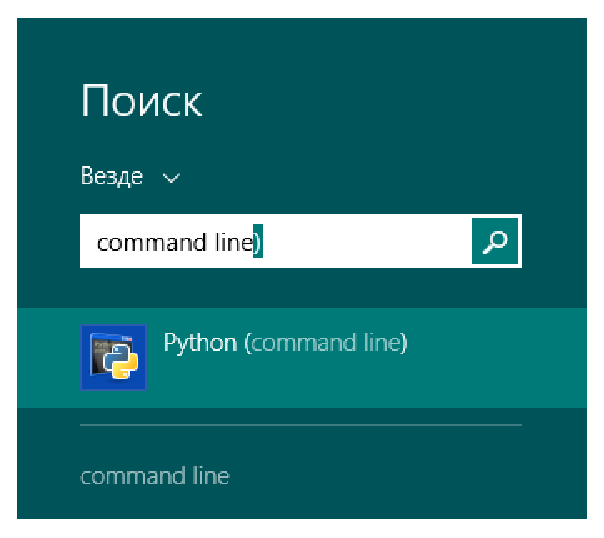
\includegraphics[width=80mm]{figure1.eps}
\end{center}
\caption{Python в меню Windows.}\label{fig1}
\end{figure}

\begin{figure}
\begin{center}
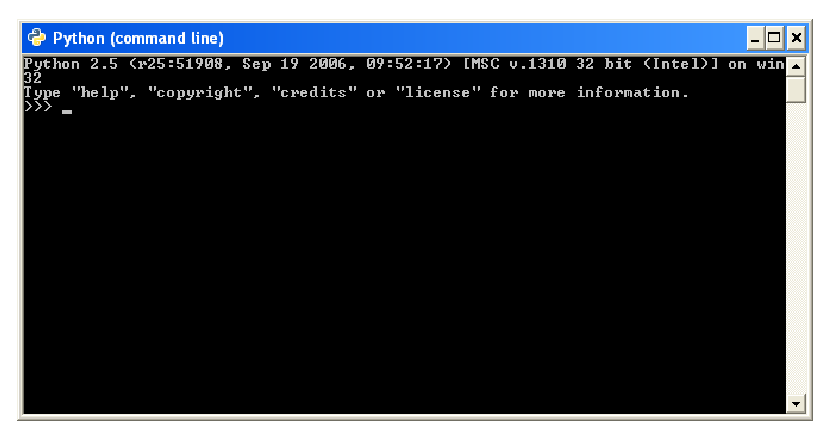
\includegraphics[width=135mm]{figure2.eps}
\end{center}
\caption{Консоль Python в Windows.}\label{fig2}
\end{figure}
\end{WINDOWS}

\begin{MAC}
В Finder, слева ты должен видеть раздел `Applications'.  Нажми на него, и затем найди программу под названием `Terminal' (она вероятно будет в папке под названнием`Utilities').
Нажми на `Terminal' и, когда он запустится, введи 'python' и нажми клавишу 'enter'.  Ты должен теперь смотреть на окно, которое выглядит как на картинке~\ref{fig3}.

\begin{figure}
\begin{center}
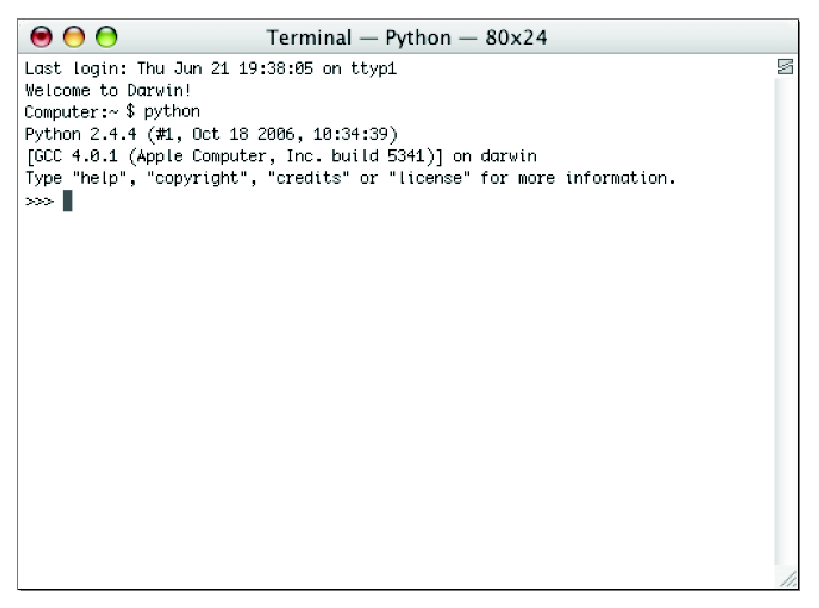
\includegraphics[width=85mm]{figure3.eps}
\end{center}
\caption{Консоль Python в Mac OSX.}\label{fig3}
\end{figure}
\end{MAC}

\begin{LINUX}
Спроси маму или папу, какую именно программу терминала тебе следует использовать (он может называться одной из этих: `Konsole', `rxvt', `xterm' или любая другая из десятка других---поэтому тебе скроее всего нужно спросить).  Запусти программу терминала и напечатай `python' (без кавычек), и нажми enter.  Ты должен увидеть что-то похожее на картинку~\ref{fig4}.

\begin{figure}
\begin{center}
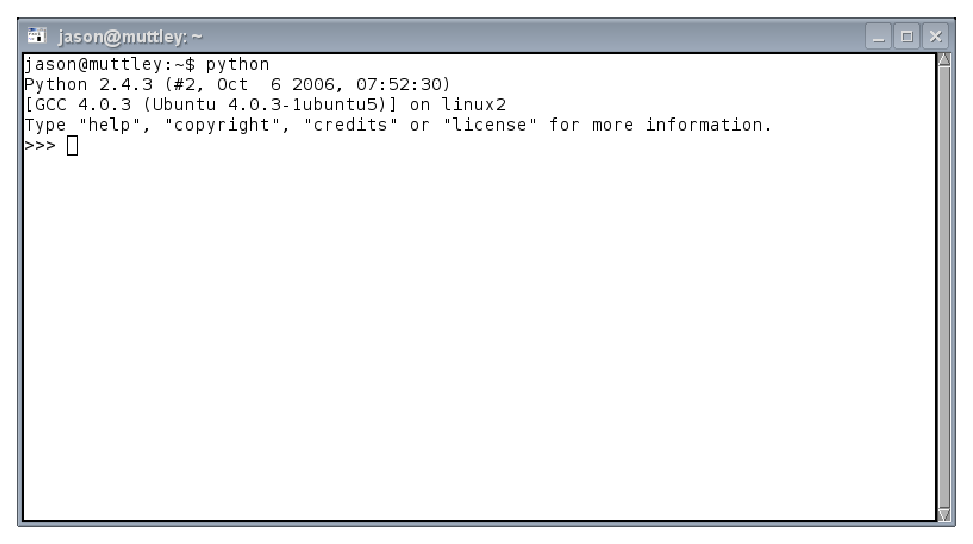
\includegraphics[width=80mm]{figure4.eps}
\end{center}
\caption{Консоль Python в Linux.}\label{fig4}
\end{figure}
\end{LINUX}

\subsection*{\color{BrickRed}Если ты обнаружил, что они не прочитали раздел в начале книги$\ldots$}

$\ldots$потому что чего-то не хватает, когда ты пытаешься следовать этим инструкциям---тогда отлистай в начало книги, подсунь её им под нос пока они читают свои книжки, и с надеждой повторяй ``пожалуйста пожалуйста пожалуйста пожалуйста'', снова и снова, пока это не начнёт надоедать, это должно сработать, если у тебя возникают сложности убедить их встать с дивана.  Конечно, кроме этого, ты можешь сам открыть начало книги и самостоятельно выполнить указанные там инструкции, чтобы установить Python.

\section{Твоя первая программа на Python}

Надеюсь, если ты дочитал до это места, у тебя уже получилось запустить консоль Python, которая позволяет выполнять программы и команды языка Python. Когда ты впервые запустишь эту консоль (или после того, как наберешь в ней первую команду), ты увидишь то, что называется `приглашение' (англ. prompt).  В консоли Python \index{Python console} приглашение выглядит в виде трёх треугольников или знаков больше ($>$), указывающих вправо:

\begin{listing}
\begin{verbatim}
>>>
\end{verbatim}
\end{listing}
Если ты составишь достаточное количество команд Python вместе, у тебя получится программа, которую ты сможешь запускать не только в консоли$\ldots$ но мы пока не станем усложнять, а будем вводить команды прямо в консоли, после приглашения ($>>>$). Так почему бы уже не начать, напечатав следующую команду (если нужно, спроси у родителей, как переключать ввод между русским и английским):

\begin{listing}
\begin{verbatim}
print("Привет Мир")
\end{verbatim}
\end{listing}

Убедись, что ты добавил кавычки (вот эти: $"$ $"$) и нажад ввод (Enter) в конце строки. Скорее всего ты увидишь что-то подобное:

\begin{listing}
\begin{verbatim}
>>> print("Привет Мир")
Привет Мир
\end{verbatim}
\end{listing}

Снова появится приглашение, давая тебе понять, что консоль Python готова принимать новые команды.

\noindent
Поздравляю! Ты только что создал свою первую программу на языке Python.  \code{print} это функция, которая выводит в консоль всё, что находится у неё между скобок--мы ещё не раз будем её использовать.

\section{Твоя вторая программа на Python$\ldots$опять тоже самое?}

Программы Python не были бы так полезны если бы тебе приходилось печатать её команды каждый раз, когда ты хотел бы что-то сделать---или если бы ты написал команду для кого-нибудь, и ему пришлось бы напечатать её перед тем, как начать использовать.

Текстовый редактор, который ты, возможно, используешь для своих школьных заданий, содержит, где-то от 10 до 100 миллионов строк кода. В зависимости от того, как много строк ты напечатаешь на одном листе (и будешь ли печатать с двух сторон или с одной), получилось бы 400,000 страниц$\ldots$ или стопка бумаги 40 метров высотой.
Просто представь, чтобы отвезти эту программу из магазина домой, потребовалось бы несколько ходок до машины, чтобы перенести так много бумаги$\ldots$

$\ldots$и тебе лучше надеятся, чтобы не было сильного ветра, пока ты носишь эти стопки бумаги. К счастью, есть альтернативный способ всему этому печатанию---иначе никто ничего не смог бы сделать.

\begin{center}
\includegraphics*[width=85mm]{pullinghair.eps}
\end{center}

\begin{WINDOWS}
Открой Блокнот (нажми на окошко внизу слева и начни печатать ``блокнот'', а потом нажми мышкой на найденную программу Блокнот), и напечатай команду print точно так же, как ты её печатал до этого в консоли:

\begin{listing}
\begin{verbatim}
print("Привет Мир")
\end{verbatim}
\end{listing}

Click on the File menu (in Notepad), then Save, and when prompted for a file name, call it \emph{hello.py} and save it on your Desktop. Double-click on the icon for hello.py on your Desktop (see Figure~\ref{fig5}) and for a brief moment a console window will appear.  It will vanish too quickly for you too make out the words, but Hello World will have been printed to the screen for a fraction of a second---we'll come back to this later and prove that it did.\\

\begin{figure}
\begin{center}

\includegraphics[width=58mm]{figure5.eps}
\end{center}
\caption{hello.py icon on the Windows Desktop.}\label{fig5}
\end{figure}
\end{WINDOWS}

\begin{MAC}
Open up the Text Editor by clicking on its icon.  It may be in the Dock at the bottom of the screen \includegraphics*[width=12mm]{textedit-icon.eps}, or look for this icon \includegraphics*[width=19mm]{textedit-icon2.eps} in the Applications list in Finder.  Type the print command exactly as you typed it into the console earlier:

\begin{listing}
\begin{verbatim}
print("Hello World")
\end{verbatim}
\end{listing}

Click on the File menu, then click on Save, and when you are prompted for a file name, call it hello.py and save it into your home directory (your home directory is on the left under Places--ask Mum or Dad to point it out for you).

Open the `Terminal' application again--it will automatically start up in your home directory--and type the following:

\begin{listing}
\begin{verbatim}
python hello.py
\end{verbatim}
\end{listing}

You should see Hello World written to the window exactly as it was when you typed the command in the Python console.

\end{MAC}

\begin{LINUX}
Open a text editor (again you might have to ask Mum or Dad which one to use), then type the print command exactly as you typed it into the console:

\begin{listing}
\begin{verbatim}
print("Hello World")
\end{verbatim}
\end{listing}

Click on the File menu, then Save, and when prompted for a file name, call it hello.py and save it in your Home folder (there might be an icon called `Home' somewhere in the Save dialog box).  Next open up the terminal application (again Konsole, rxvt, etc... what we used earlier), and type:

\begin{listing}
\begin{verbatim}
python hello.py
\end{verbatim}
\end{listing}

You should see Hello World written to the window exactly as it was when you typed the command in the Python console (see Figure~\ref{fig9}).

\begin{figure}
\begin{center}
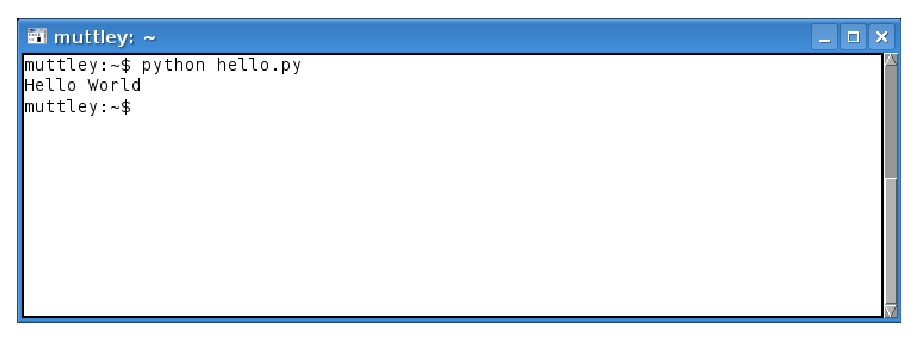
\includegraphics[width=75mm]{figure9.eps}
\end{center}
\caption{Running a python program from a text file on Linux.}\label{fig9}
\end{figure}
\end{LINUX}

So you can now see that the nice people who created Python, have kindly saved you from having to type the same thing over and over and over and over and over again.  Like they did back in the 1980's.  No, I'm serious---they did.  Go and ask your Dad if he ever owned a ZX81 when he was younger?\\

\noindent
If he did you can point at him and laugh.\\

\noindent
Trust me on this one.  You won't get it.  But he will.\footnote{The Sinclair ZX81, released in the 1980's was one of the first affordable home computers.  A number of young boys and girls were driven completely mad, typing in the code for games printed in popular ZX81 magazines---only to discover, after hours of typing, that the darn things never worked properly.}

\noindent
\emph{Be prepared to run away though.}

\subsection*{\color{BrickRed}The End of the Beginning}

Welcome to the wonderful world of Programming.  We've started really simply with a ``Hello World'' application---everyone starts with that, when they're learning to program.
In the next chapter we'll start to do some more useful things with the Python console and then look at what goes into making a program.

\newpage